\chapter{Réalisations}
%Si besoin, vous pourriez structurer le reste du rapport en plusieurs parties et non une seule. La ou les parties devraient elles-mêmes êtres structurées en plusieurs sous-sections au sein d'une même partie. Dans tous les cas, la logique du plan doit apparaître clairement.

%Travaillez les liaisons pour aboutir à une lecture fluide. Voici un exemple (un peu exagéré) : "Après avoir inventorié les technologies disponibles dans la section précédente, cette section est consacrée aux expérimentations que nous avons menées avec chacune d'elles. Ce travail nous permettra de sélectionner les technologies retenues, présentées dans la section suivante."

%Présentez votre réflexion et vos choix, qui devraient être justifiés. Examinez rapidement les autres alternatives.

%Sélectionnez les détails pertinents et laissez les autres en annexe. Allez du général au particulier. Evitez de présenter un catalogue des fonctions développées.
Le sujet de mon stage étant large, très tôt j'ai dû me concentrer sur plusieurs tâches puis rapidement m'atteler à plusieurs réalisations afin d'assurer au mieux ma fonction. Nous verrons donc dans ce chapitre, pour chacune de ces différentes réalisations, les besoins auxquels il fallait répondre, les choix qui ont été fait et les différentes difficultés rencontrées.

\section{Conception d'un processus de production et de gestion des rapports de test}
%QQchose ?
\subsection{État des lieux}
Dans un premier temps, une présentation du contexte initial est indispensable. Au sein de l'équipe \gls{TC}, il existe différentes phases de test, dont l'organisation correspond au cycle en V du projet (cf. Annexe I) :
\begin{itemize}
\item \textbf{FAT} : Factory Acceptance Test, test d'acceptation usine consistant à inspecter le système dans l'usine avant livraison. Pendant le FAT, les performances du système sont contrôlées, généralement en collaboration avec le client.
\item \textbf{iFAT} : Integrated Factory Acceptance Test, test d'acceptation intégré usine consistant à contrôler le fonctionnement des différents équipement ensemble.
\item \textbf{\gls{StAT}} : Stand Alone Test, test unitaire, où  l'équipement testé est isolé de toute interaction durant le test, afin de restreindre les critères du test à son fonctionnement autonome.
\item \textbf{\gls{SIT}} : Site Integration Test, test d'intégration, ayant pour but de détécter les erreurs non détéctables pendant les test unitaires. Ce type de test consiste à assembler différents composants afin de tester leur fonctionnement dans l'ensemble.
\item \textbf{\gls{E2E}} : End to End Test, test bout en bout ayant pour but de vérifier si un système se comporte comme prévu du début à la fin. Le testeur doit se mettre dans le rôle d’un utilisateur et effectuer les tests comme s’il utilisait véritablement l’outil mis à sa disposition.
\end{itemize}

Nous nous concentrerons ici sur les phases \gls{StAT}, \gls{SIT}, \gls{E2E}. 

Pour chaque sous-système du projet, 3 procédures de test ont été rédigées, une par phase de test. 

Ainsi, si une localisation du projet abrite 3 sous-systèmes nécessitant d'être testés, il y aura 9 tests à effectuer dans cette localisation.

Ensuite, chaque test doit être formalisé par un rapport de test constitué de la manière suivante : 

\begin{itemize}
\item Une première page que l'on appelle ITR, qui permet d'identifier le rapport (numéro unique), d'identifier le test (localisation, phase, système, date), identifier le statut (accepté avec, sans réserves ou refusé), résumer les observations et réserves des 3 parties et consigner leurs signatures.
\item Les pages suivantes sont les \gls{TestCases}, en français les scénarios de test, qui permettent de simuler plusieurs situations d'utilisation des systèmes de manière à prouver leur conformité vis à vis de toutes les exigences du cahier des charges.
\begin{itemize}
\item Chaque \gls{TestCases} est composé de une ou plusieurs étapes qui elles mêmes sont reliées à une ou plusieurs exigences.
\end{itemize}
\end{itemize}

Parmi ces exigences, certaines sont liées à la sécurité, dans le cadre des \gls{RAMS}, et sont indexées dans un document appelé le \gls{SC}. Ces exigences liées à la sécurité sont séparés en deux \gls{SIL}, ou niveaux de criticité : SIL0, le plus faible et SIL2 le plus élevé.

Une fois ce contexte clarifié, nous avons pu entreprendre l'élaboration du processus et c'est le sujet de la prochaine section.

\subsection{Première version}

Après l'analyse exposée précédemment, nous avons travaillé conjointement avec mon maître de stage sur une première version du processus que voici :

\begin{center}
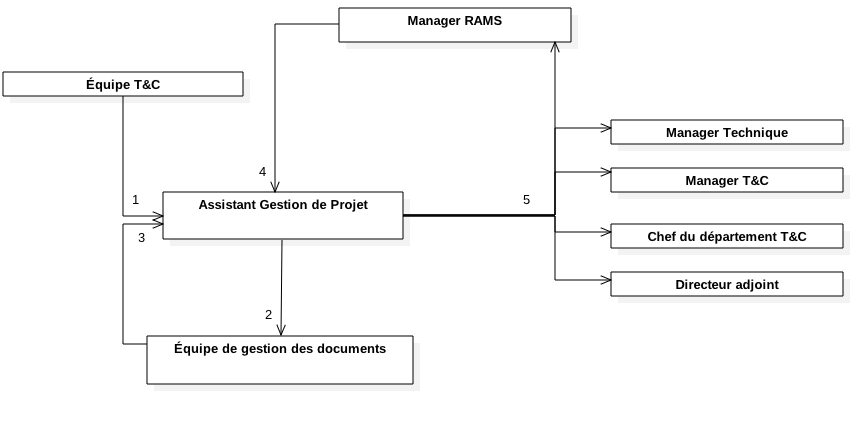
\includegraphics[height=7cm]{ressources/images/figures/Workflow1.png}
\end{center}


\begin{itemize}
\item \textbf{1.} Tout d'abord, l'équipe \gls{TC} effectue les différentes inspections et produit les rapports de test en remplissant les formulaires correspondant sur \gls{SnagR}.  
\item \textbf{2.} Ensuite j'extraie les données de \gls{SnagR} (nous reviendrons sur ce point dans la prochaine partie) et les importe dans un fichier Excel afin de les exploiter. J'exporte les rapports au format pdf et les envoie à l'équipe de gestion des documents.
\item \textbf{3.} Cette dernière importe les rapports sur \gls{Mezzoteam} afin de rendre ces preuves accessibles à tout les membre du projet et les importe aussi sur \gls{e-TOL} pour que les membre de l'équipe Thales offshore puissent les consulter. Une fois l'importation terminée, l'équipe me fournit les références de ces documents afin que je les ajoutes à ma base de donnée.
\item \textbf{4.} Le manager \gls{RAMS} et son équipe me fournissent des mises à jours concernant les exigences liées à la sécurité afin que je puisse actualiser mon fichier car les rapports devant servir de preuve pour ces dernières nécessitent d'être suivis de manière prioritaire. En effet, le futur opérateur refusera de commencer la période de formation de ses employés à l'exploitation du système tant qu'il n'aura pas la preuve de la conformité du projet vis à vis de ces exigences.
\item \textbf{5.} Enfin, il me faut communiquer les résultats aux différents managers sous forme de \gls{KPI}, courbes et outils d'aide à la décision. Nous reviendrons plus tard sur ce point.
\end{itemize}

Ce processus fut mis en place et appliqué durant le premier mois de mon stage, mais il fallu rapidement l'adapter.

\subsection{Évolution du processus}

En effet, aux vues des différentes responsabilités que l'on m'a confié à partir du second mois, j'ai du intégrer à ce processus de nouvelles étapes. 
Voici ci-dessous la matrice de responsabilité de notre projet suivant la méthode RACI. Dans cette matrice, le R signifie responsable et désigne la personne qui exécute l'action, le A désigne la personne qui approuve l'action, le C une personne consultée et le I une personne devant être tenue informée.

\begin{center}
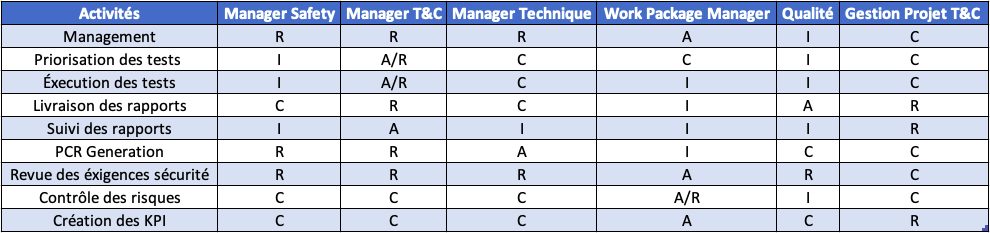
\includegraphics[height=4cm]{ressources/images/figures/RACI.png}
\end{center}

Ainsi, j'ai dû intégrer au processus de nouveaux acteurs ainsi que de nouvelles interactions. 

\begin{center}
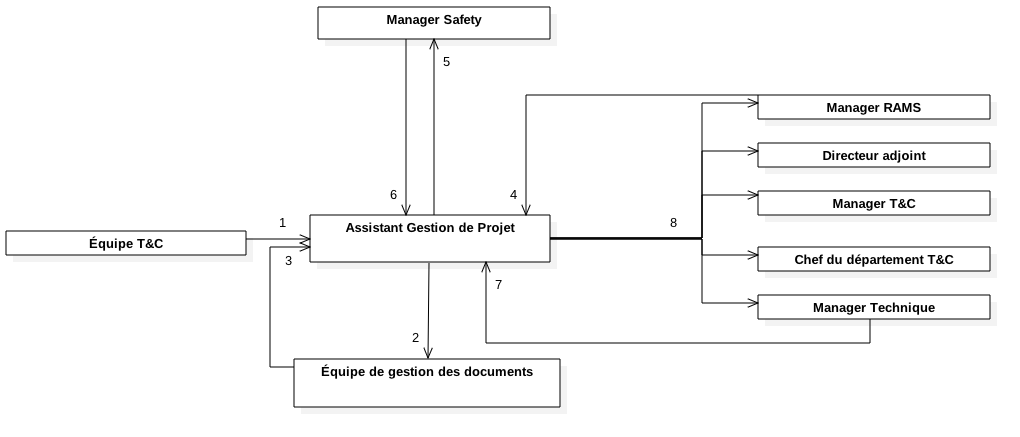
\includegraphics[height=7cm]{ressources/images/figures/Workflow2.png}
\end{center}


\begin{itemize}
\item \textbf{Étapes 1 à 4.} Identiques à la première version du processus.
\item \textbf{5.} Après avoir vérifié que les exigences liées à la sécurité étaient bien à jour, il me fallait fournir au manager sécurité les données nécésssaires à la vérification de la conformité des systèmes. Je devais donc lui fournir, pour chaque exigence déjà vérifiée lors d'un test, la référence du rapport de ce test ainsi que celles des \gls{TestCases} permettant de vérifier la conformité de l'exigence.
\item \textbf{6.} Ensuite, le manager sécurité devait spécifier, pour chaque \gls{TestCases} lié à une exigence sécurité, si il était conforme ou non, et le cas échéant, il devait générer une \gls{PCR} afin de notifier ce défaut aux autres équipes.
\item \textbf{7.} Après cela, je collectais, auprès du manager technique (et de son équipe), les différents facteurs limitant retardant l'execution de certains test, afin de pouvoir, à l'étape suivante, réaliser des outils d'aide à la décision.
\item \textbf{8.} Comme précédemment, il fallait enfin communiquer les résultats aux managers.
\end{itemize}


Dans un soucis de synthèse, la version du processus final exposée ci-dessus est une version simplifiée, mais les étapes principales y sont représentées. 
Au cours de la prochaine partie, nous allons nous intéresser à la réalisation de la deuxième étape du processus : l'extraction des données. 

\section{Mise au point d'un outil d'extraction de données }
%QQchose ?

\subsection{Les motivations}
1500 rapports
Plus de 15 000 TC (formulaire)
Plus de 60 000 steps (étapes)
Après avoir importé manuellement les données des premiers rapports, .. tourné vers SnagR :
Présentation des activités
Problème de cohérence
=> KPI Fausse
Absence de validation des données
Exportation des données limitées
Donc besoin d'implémenter moi même
\gls{scraping}

\subsection{Les différentes fonctionnalités de l'outil}
Sauvegarde complète
Actualisation en deux étapes
\subsection{Les choix techniques}
DB, Access, powerbi ou excel ?
=> Limitations dues au caractère sensible des données, process beaucoup trop long

Pandas

Multi thread ou multi process ?
=> 
Temps d'éxécution : 1h30 => 5 min (laisser qq latences)

Python 3 ou le choix de la pérénité
=> 2to3

\section{Communication sur l'avancement du projet}
\subsection{Organisation des données}
Séparation
Séléction
\subsection{Communication interne}
Outils d'aide à la décision
KPI
S-Curves
Syncronisation avec le Testing pour plus de cohésion
\subsection{Communication avec le client}
Difficultés de la position de Thales


\section{Formation et transmission}
\subsection{Sensibilisation des membre de l'équipe }
Sensibilisation à l'importance des rapports
Formation à la validation des données (doc, convention de nommage)
\subsection{Tuilage}
Doc
Etat de l'avencement
Vidéos tutorielles


